\documentclass[a5paper]{article}
\usepackage[a5paper, top=8mm, bottom=8mm, left=8mm, right=8mm]{geometry}

\usepackage{polyglossia}
\setdefaultlanguage[babelshorthands=true]{russian}

\usepackage{fontspec}
\setmainfont{FreeSerif}
\newfontfamily{\russianfonttt}[Scale=0.7]{DejaVuSansMono}

\usepackage[font=scriptsize]{caption}

\usepackage{amsmath}
\usepackage{amssymb,amsfonts,textcomp}
\usepackage{color}
\usepackage{array}
\usepackage{hhline}
\usepackage{cite}
\usepackage{textcomp}

\usepackage[hang,multiple]{footmisc}
\renewcommand{\footnotelayout}{\raggedright}

\PassOptionsToPackage{hyphens}{url}\usepackage[xetex,linktocpage=true,plainpages=false,pdfpagelabels=false]{hyperref}
\hypersetup{colorlinks=true, linkcolor=blue, citecolor=blue, filecolor=blue, urlcolor=blue, pdftitle=1, pdfauthor=, pdfsubject=, pdfkeywords=}

\newlength\Colsep
\setlength\Colsep{10pt}

\usepackage{tabu}

\usepackage{graphicx}
\usepackage{indentfirst}
\usepackage{multirow}
\usepackage{subfig}
\usepackage{footnote}
\usepackage{minted}

\newcommand{\todo}[1] {
\begin{center}\textcolor{red}{TODO: #1}\end{center}
}

\newcommand{\attribution}[1] {
    \vspace{-5mm}\begin{flushright}\begin{scriptsize}%\textcolor{gray}
    {\textcopyright\, #1}\end{scriptsize}\end{flushright}
}

\sloppy
\pagestyle{plain}

\title{Лекция 6/Практика 4: Структурные шаблоны}
\author{Юрий Литвинов\\\small{y.litvinov@spbu.ru}}
\date{14.04.2022}

\begin{document}

\maketitle
\thispagestyle{empty}

\section{Введение}

\subsection{Зачем паттерны и зачем их изучать?}

Шаблоны (или паттерны) проектирования --- это набор стандартных решений, применяемых в типичных ситуациях. Популяризованы они были в середине 90-х годов знаменитой книгой <<Приёмы объектно-ориентированного проектирования. Паттерны проектирования>> Э. Гамма, Р. Хелм, Р. Джонсон, Д. Влиссидес (так называемая <<банда четырёх>>, известные популяризаторы объектно-ориентированного программирования). В академической среде про паттерны начали говорить ещё раньше (и вообще, всё пошло из городской архитектуры, К. Александера <<Язык шаблонов. Города. Здания. Строительство>> 1977 года), но по-настоящему актуальны они стали в связи со взрывным развитием объектно-ориентированных языков в 90-х и появлением Java (хотя первое издание книги использовало язык Smalltalk). В конце 90-х и в 2000-х на паттерны чуть ли не молились, вышло несколько переизданий оригинальной книги и десятки других книг, курсов и сайтов с красивыми картинками, что хорошая новость, потому что найти материал для подготовки по этой теме ничего не стоит (и я бы даже рекомендовал не читать этот конспект, а найти на просторах интернета что-нибудь, что вам больше понравится --- современное издание книги <<банды четырёх>> вполне подойдёт, можно и что-то другое, но что-то про паттерны прочитать точно надо). 

Сейчас, тем не менее, сообщество сходится на том, что паттерны проектирования предназначены скорее для борьбы с недостатками Java и для современных языков не так актуальны. И действительно, с 90-х годов языки (даже консервативная Java) успели эволюционировать, некоторые паттерны оказались встроенными в язык (например, паттерн <<Наблюдатель>> реализован в C\# с помощью механизма событий), некоторые оказались больше не так полезны (например, повсеместное использование лямбда-функций делает паттерн <<Стратегия>> несколько избыточным). Кроме того, можно сказать, что популярные языки программирования постепенно смещаются в сторону функциональной парадигмы, а она паттерны проектирования вообще отрицает (хотя функциональные паттерны тоже, конечно, есть --- например, Continuation Passing Style и монады, это, по сути, паттерны). Тем не менее, паттерны проектирования до сих пор считается приличным знать любому адекватному программисту, про них практически всегда спрашивают на собеседованиях, так что в этом курсе на паттерны проектирования отводится аж три пары. На самом деле, знать паттерны полезно даже если ими не пользоваться --- они очень хорошо открывают глаза на объектно--ориентированное программирование и <<тактическую>> архитектуру, показывают ряд интересных приёмов.

\subsection{Что такое паттерны}

Итак, следуя Википедии, \textit{паттерн проектирования} --- это повторяемая архитектурная конструкция, представляющая собой решение проблемы проектирования в рамках некоторого часто возникающего контекста\footnote{Шаблон проектирования, URL: \url{https://ru.wikipedia.org/wiki/Шаблон_проектирования}}. Паттерны

\begin{itemize}
    \item имеют имя, что позволяет унифицировать терминологию и упростить общение между разработчиками --- гораздо проще сказать <<Тут реализован паттерн ``Состояние''>>, чем долго объяснять, как он работает;
    \item широко известны, так что если вы говорите <<Тут реализован паттерн ``Состояние''>>, можно смело рассчитывать, что вас поймут;
    \item изложены структурированно и в удобной для изучения форме, что помогает переиспользованию знаний и быстрому введению молодых специалистов в суть дела;
    \item подходят для решения целого класса проблем, которые возникают в разных предметных областях при программировании на разных языках --- так что они достаточно универсальны, чтобы их стоило изучать на общем курсе по архитектуре.
\end{itemize}

При этом паттерны не:

\begin{itemize}
    \item не конкретный рецепт или указания к действию --- паттерны скорее стоит понимать как идеи или красивые приёмы, которые можно использовать или от которых можно отталкиваться при проектировании;
    \item не приёмы использования конкретных языков --- бывают языковые идиомы, например, RAII\footnote{Resource Acquisition Is Initialization, идиома, связывающая управляемые ресурсы типа открытых файлов или сетевых соединений с временем жизни объекта, который их представляет в программе} в C++, это не паттерны. Паттерны должны быть применимы в рамках целой парадигмы программирования, вне зависимости от языка.
\end{itemize}

Начинающие проектировщики часто понимают паттерны именно как конкретные рецепты или даже как просто что-то хорошее, что делает любую архитектуру лучше --- в своё время был популярен анекдот про то, как кто-то написал Гамме письмо, что он уже использовал в своём проекте 12 паттернов из книжки, и может ли ему Гамма подсказать, куда вставить оставшиеся. Это очень неправильная точка зрения, паттерн --- это именно идея, хорошо зарекомендовавшая себя в некоторых распространённых ситуациях. Идею можно по-разному реализовать, можно модифицировать, и часто описания паттернов включают в себя рассуждения по поводу разных вариантов. Так что бояться отклониться от шаблона не надо --- единственное, что в рамках этого курса всё-таки стоит научиться делать как положено, а уже потом, как паттерны будут освоены, менять их и подстраивать под конкретные ситуации.

Паттерны условно делятся на \textit{структурные}, \textit{поведенческие} и \textit{порождающие}. Структурные паттерны по идее описывают особенности структуры во время компиляции, поведенческие занимаются поведением системы во время выполнения, а порождающие описывают разные способы создавать сложные группы объектов. Однако разделение это очень условно, поэтому мы не будем его строго придерживаться, и не рекомендую пытаться запомнить, какой паттерн к какой группе относится: например, в книге <<Банды Четырёх>> паттерн <<Декоратор>> относится к структурным, а паттерн <<Стратегия>> к поведенческим, хотя они очень похожи по смыслу. Тем не менее, в литературе такое разделение встречается часто.

\subsection{Место паттернов в архитектуре}

В одной из презентаций проф. N. Medvidovic из USC была картинка, проясняющая место паттернов проектирования в архитектуре, она воспроизведена на рис~\ref{image:patterns}.

\begin{figure}
    \begin{center}
        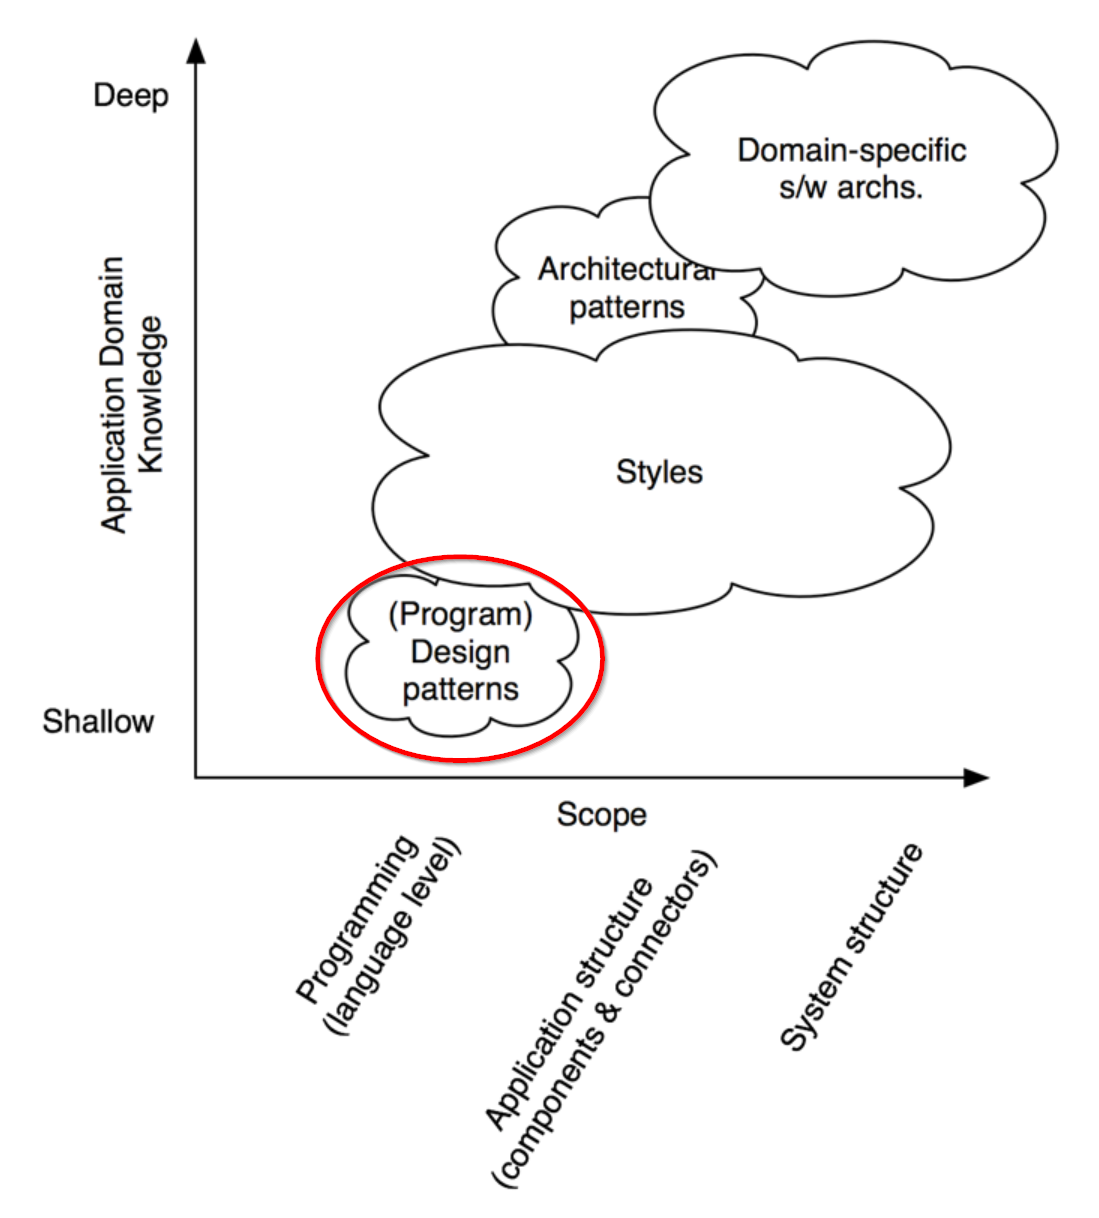
\includegraphics[width=0.55\textwidth]{architecturalStylesPatternsHighlighted.png}
    \end{center}
    \caption{Место паттернов проектирования в архитектуре.}
    \label{image:patterns}
\end{figure}

Паттерны проектирования не специфичны для предметной области и могут успешно применяться в самых разных контекстах, вместе с тем они предлагают тактические архитектурные решения, не затрагивая общую архитектуру приложения или подсистемы. Поэтому паттерны проектирования занимают левую нижнюю часть картинки. На самом деле, паттерны проектирования можно понимать как границу между программированием и архитектурой --- если вы детализировали архитектуру до уровня, что понятно, какие паттерны где применять, стоит остановиться и большую детализацию отложить на этап реализации. Если в команде есть выделенный архитектор, то использование паттернов ему ещё может быть интересно, а вот как именно они реализуются --- он может доверить программистам.

В этом курсе мы начнём с паттернов и поговорим также и про архитектурные стили и (немного) про архитектурные паттерны. А вот про предметно-ориентированные архитектуры говорить не будем, потому что они актуальны только в рамках конкретной предметной области --- например, существуют референсные архитектуры для автомобильного или аэрокосмического программного обеспечения, они очень подробно описывают структуру приложений, протоколы коммуникации и т.п., и следование им обязательно для успешной сертификации (которая в большинстве случаев обязательна в этих областях). Поскольку вероятность того, что кто-то из слушателей этого курса столкнётся с какой-то конкретной референсной архитектурой, минимальна (и поскольку каждая из них заслуживает отдельного курса), мы их обсуждать не будем.

\subsection{Модельный пример}

Дальше мы перейдём наконец к конкретным паттернам. Изложение в большинстве случаев будет, следуя книге <<банды четырёх>>, вестись на примере текстового редактора. Положим, мы хотим разработать свой текстовый редактор с нуля, причём это должен быть WYSIWYG\footnote{What You See Is What You Get}-редактор --- редактор, где страница при редактировании выглядит так, как она будет напечатана или сохранена (наподобие Microsoft Word и в противоположность TeX, где редактируется специальная разметка, а для получения результата требуется компиляция). Для того, чтобы написать такой редактор, нам потребуется решить ряд архитектурных вопросов.

\begin{itemize}
    \item Как представляется внутри редактора структура документа? Документ ведь надо не только выводить на экран, но и эффективно хранить в памяти, так, чтобы эффективно выполнять разные операции (типа редактирования, форматирования и т.д.).
    \item Как будет работать форматирование документа, в смысле размещение текста на странице, выравнивание и т.д.? Поскольку у нас WYSIWYG-редактор, нам важна скорость работы, но также важно и качество результата, так что, как и всегда, имеются конфликтующие требования.
    \item Как мы реализуем красивый и удобный интерфейс пользователя? Поскольку у нас курс по архитектуре, вопросы типа размещения и цвета кнопок нас не волнуют, но нам надо придумать архитектуру такой, чтобы дизайнер мог легко воплотить самые разные свои идеи.
    \item Как поддержать разные стандарты внешнего облика программы? В разных операционных системах look and feel программы по традиции свой, хочется безболезненно приспосабливаться под разные стандарты.
    \item Как поддержать команды, которые пользователь может выполнять с редактором, операции отмены и повторения команд? Кажется, что проблема мелкая, но если о ней заранее не подумать, встроить поддержку undo/redo в готовый редактор может оказаться очень сложно --- реализовать для каждой из десятков операций undo/redo отдельно можно с ума сойти.
    \item Как будут выполняться разные аналитические операции типа проверки правописания и расстановки переносов? Сами операции могут быть весьма нетривиальны, не хочется их реализовывать в одной общей куче кода.
\end{itemize}

\section{Паттерн <<Декоратор>>}

\subsection{Мотивирующий пример}

Итак, проектируем текстовый редактор. Мы хотим сделать поддержку всяких украшательств пользовательского интерфейса, типа рамок вокруг области ввода текста, и полосы прокрутки. При этом хочется, чтобы пользователи могли включать-выключать по опции разные элементы пользовательского интерфейса, а в случае с полосой прокрутки --- иметь возможность и автоматически её добавлять/убирать в зависимости от количества текста. Причём так, чтобы другие части редактора даже не знали про то, есть там где-то полосы прокрутки или нет.

Будем считать, что всё, что можно нарисовать на экране --- наследник класса Glyph, в том числе символы, картинки, строки (собранные из символов), колонки на странице (собранные из строк), сами страницы с текстом. Первое решение, которое приходит в голову --- сделать ещё одного наследника Glyph, <<страница с текстом в рамке>>, а потом ещё одного, <<страница с текстом с полосой прокрутки>>. Но это не удобно, потому что вдруг мы захотим страницу и в рамке, и с полосой прокрутки. Да и поскольку наследование --- структура времени компиляции, менять во время выполнения обрамлённый текст на необрамлённый очень сложно. Поэтому наследование мы использовать не хотим, а хотим использовать композицию. 

Идея с наследованием от Glyph на самом деле всё-таки не так уж и плоха: мы можем сделать классы <<Рамка>> и <<Полоса прокрутки>> глифами, что позволит им вкладываться друг в друга и нисколько не противоречит архитектуре (всё, что можно нарисовать на экране --- наследник класса Glyph, а полосу прокрутки определённо можно нарисовать на экране). Это имеет тот побочный эффект, что рамки и полосы прокрутки могут появляться где угодно в тексте, а не только вокруг страницы --- но, возможно, это и не плохо, особенно в случае с рамками. Такой приём в книжке <<Банды Четырёх>> называется <<прозрачное обрамление>>, поскольку для всего внешнего мира глифы с рамками и без неразличимы, то же с полосами прокрутки.

Чтобы реализовать эту идею, добавим в нашу архитектуру класс MonoGlyph: абстрактный класс с ровно одним сыном, он будет базовым для всех видов <<обрамлений>>:

\begin{center}
    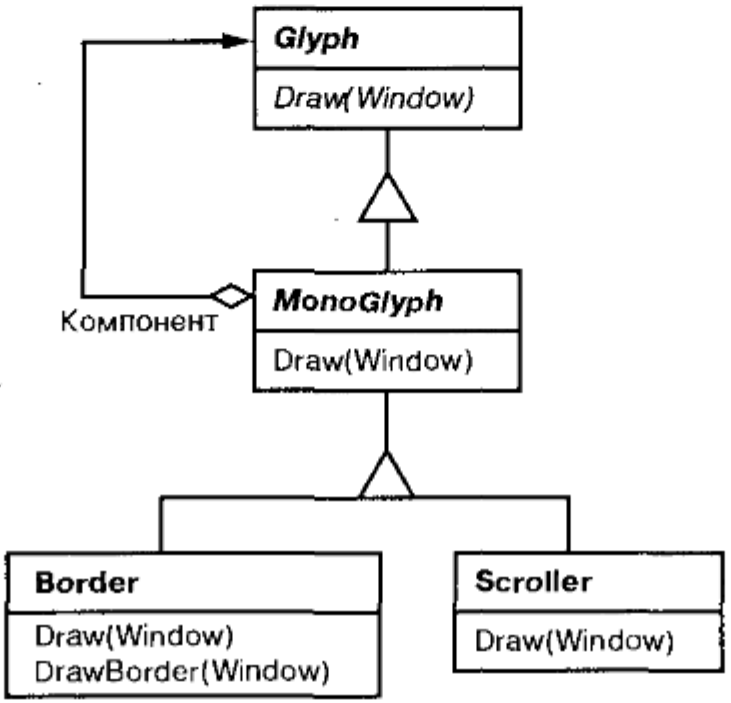
\includegraphics[width=0.4\textwidth]{monoglyph.png}
    \attribution{Э. Гамма и др., Приемы объектно-ориентированного проектирования}
\end{center}

Во время выполнения структура объектов может выглядеть так:

\begin{center}
    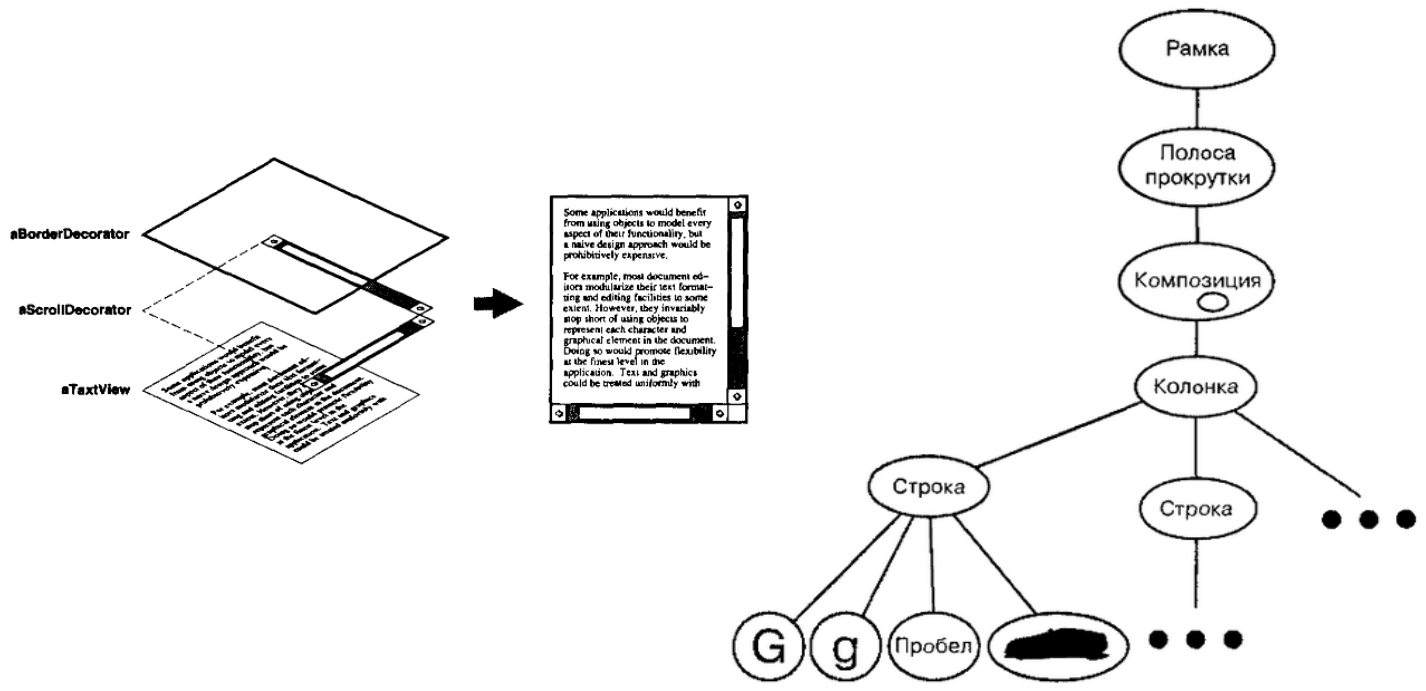
\includegraphics[width=0.9\textwidth]{glyphStructure.png}
    \attribution{Э. Гамма и др., Приемы объектно-ориентированного проектирования}
\end{center}

Эта структура позволяет вкладывать один элемент оформления в другой, что интересно ещё и тем, что в зависимости от того, в каком порядке что вкладывается, результат может быть разным. Если сначала рамка, а затем полоса прокрутки, то скроллится содержимое рамки. Если сначала полоса прокрутки, затем рамка, то рамка сама скроллится, вместе с текстом.

\subsection{Декоратор (Decorator), общая структура}

Предложенную структуру классов можно обобщить до паттерна <<Декоратор>>:

\begin{center}
    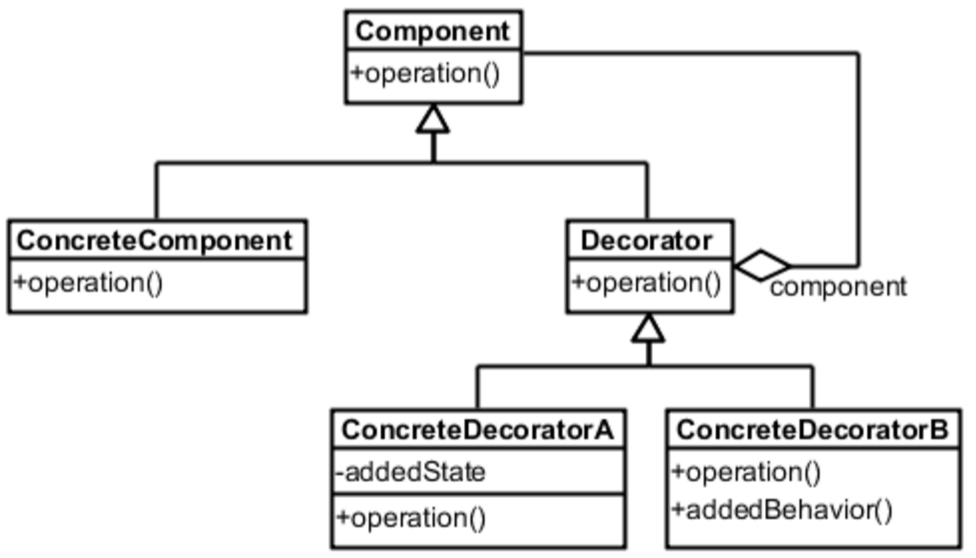
\includegraphics[width=0.55\textwidth]{decorator.png}
\end{center}

Декорировать можно как конкретные объекты (ConcreteComponent), так и другие декораторы, поэтому Decorator тоже наследуется от Component. Декоратор содержит в себе поле типа Component и вынужден (раз уж наследуется) определять все методы Component. Те, которые ему не интересны, он просто пересылает декорируемому объекту, а нужные методы (типа метода отрисовки в нашем примере с редактором) может переопределять. Или добавлять новые --- тогда те, кто ничего не знают про декоратор, могут пользоваться им прямо как декорируемым объектом и никогда не заметить разницы, а те, кто знает, могут сделать приведение типа и пользоваться новой функциональностью. Или новым состоянием, потому что и поля декоратор может иметь свои.

Это всё позволяет фактически менять поведение объекта во время выполнения, добавляя ему новые возможности или наоборот, удаляя их. Гораздо гибче, чем наследование, которое фиксируется во время компиляции и во время выполнения уже ничего не изменить. Возможность добавлять новое состояние и поведение позволяет не пытаться определить всё в базовом классе, а вынести часть функциональности в декораторы, про которые будут знать только те, кому эта функциональность нужна (и делать преобразования типов, что не очень объектно-ориентировано, но неплохо работает на практике). Однако за гибкость приходится платить --- во время выполнения оказывается много мелких объектов вместо одного большого, что приводит к дополнительным накладным расходам по памяти (да и по времени, лишние полиморфные вызовы не выполняются даром).

\subsection{Детали реализации}

Декоратор имеет довольно близкий паттерн <<Адаптер>>, который также оборачивает один объект в другой объект, но в <<Адаптере>> интерфейсы этих объектов не совпадают (поэтому он и <<Адаптер>> --- адаптирует один интерфейс для клиентов, которые хотят другой). Идея декоратора именно в том, чтобы реализовывать интерфейс декорируемых объектов, чтобы внешний мир думал, что декоратора вообще нет, и со структурой данных можно работать как обычно.

Это влечёт тот факт, что класс Component должен быть небольшим, во-первых, по количеству объявленных в нём методов: потому что мы замучаемся их переопределять, даже если переопределение для большинства из них --- это просто вызов метода декорируемого объекта, в одну строчку. Во-вторых, он должен быть небольшим по объёму хранимых в нём данных, потому что декоратор, наследуясь от Component, получает не только все его методы, но и все его поля --- и не использует их никак, ведь он просто перенаправляет запросы декорируемому объекту. Кстати, начинающие программисты часто путаются: меняют поле декоратору, а ничего не происходит --- потому что на самом деле с полем работает декорируемый объект, спрятанный в декораторе, а у него \textit{свой} набор полей. Поэтому в идеале Component должен быть вообще интерфейсом и никакого состояния не иметь.

Если это не так и Component --- это полноценный большой класс с кучей методов, лучше подойдёт паттерн <<Стратегия>>. Это как декоратор наоборот, он не надевается поверх объекта, а вкладывается в объект. Когда объекту надо выполнить какое-то действие, он обращается к стратегии и она делает за него работу. Но стратегия, в отличие от декоратора, требует, чтобы мы заранее знали, какие действия мы позволяем параметризовать с помощью стратегии, а какие нет, поэтому декоратор гибче. 

Ещё распространённый приём, более легковесный, чем <<Стратегия>> --- это заранее определить в Component набор точек расширения (<<hooks>> в англоязычной литературе), и вызывать их перед/после/во время выполнения действия. По умолчанию <<хуки>> просто ничего не делают, но если их переопределить (отнаследовавшись от Component или передав <<хуки>> как лямбда-функции), они могут модифицировать действие, как им захочется, вплоть до полной его отмены. Опять-таки, при написании Component надо заранее подумать о точках расширения, тогда как декоратор не требует в Component никаких изменений вовсе\footnote{Это не совсем правда: в C\# или C++ методы по умолчанию не виртуальные, так что если в Component не написано явно, что их можно переопределять, декоратор написать не получится. В Java методы по умолчанию виртуальные, так что там шансов больше, но Component может испортить авторам декоратора жизнь, используя final.}, поэтому гораздо гибче.

\section{Паттерн <<Стратегия>>}

\subsection{Мотивирующий пример}

Следующая задача в нашем текстовом редакторе --- алгоритмы форматирования текста. Хочется иметь механизм, размещающий текст на странице с учётом пожеланий пользователя, таких как количество колонок, ширина полей, размер абзацного отступа и т.д. При этом, поскольку у нас WYSIWYG-редактор, мы хотим, с одной стороны, чтобы оно работало в реальном времени, с другой стороны --- чтобы результат получался посимпатичнее. 

Продвинутые редакторы, типа TeX, учитывают даже такие параметры, как <<цвет>> документа (то есть соотношение пробелов и непробельных символов) и следят за тем, чтобы пробелы в соседних строках не выстраивались в одну колонку (чтобы текст визуально не разделялся надвое). WYSIWYG-редакторы обычно не могут себе такого позволить, поскольку форматирование вызывается после каждой напечатанной буквы, но кажется хорошей идеей дать возможность самому пользователю выбрать, получше сделать или побыстрее. Например, пока пользователь просто набирает текст, используется быстрый алгоритм форматирования, а когда уже верстает начисто, медленный, но дающий красивый результат.

Поэтому мы приходим к идее вынести алгоритм форматирования в отдельный класс, сделать для него интерфейс, и реализовать этот интерфейс несколькими разными алгоритмами. Чтобы встроить всё в систему, как обычно, отнаследуемся от класса Glyph, добавив <<псевдоглиф>> Composition:

\begin{center}
    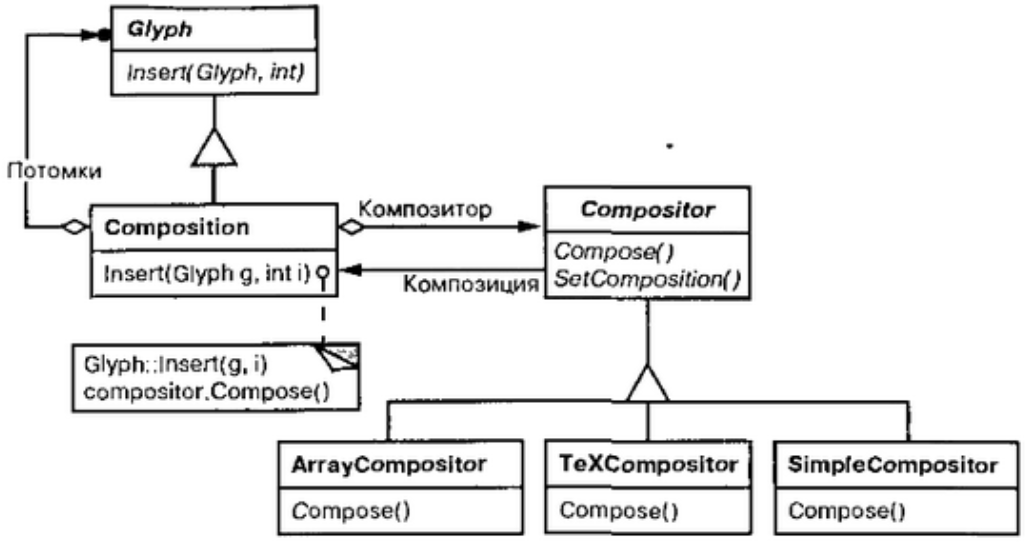
\includegraphics[width=0.7\textwidth]{compositor.png}
    \attribution{Э. Гамма и др., Приемы объектно-ориентированного проектирования}
\end{center}

Теперь, когда кто-то вызывает Insert у строки, на которую навешен Composition, она дёргает выбранный алгоритм композиции (точнее, его метод Compose), который добавляет межсимвольные интервалы, а если Insert вызван у страницы, обёрнутой в Composition, вызывается разбивка на колонки и т.д. Алгоритму нужны данные, с которыми он бы работал, поэтому у него ещё есть метод SetComposition, куда можно передать то, что ему, собственно, надо композировать.

\subsection{Стратегия (Strategy), общая структура}

Это всё обобщается до паттерна <<Стратегия>>, основное назначение которого --- инкапсуляция алгоритма в объект, так, чтобы алгоритм можно было легко прямо во время выполнения заменить, и чтобы его сложность не мешала всей остальной системе:

\begin{center}
    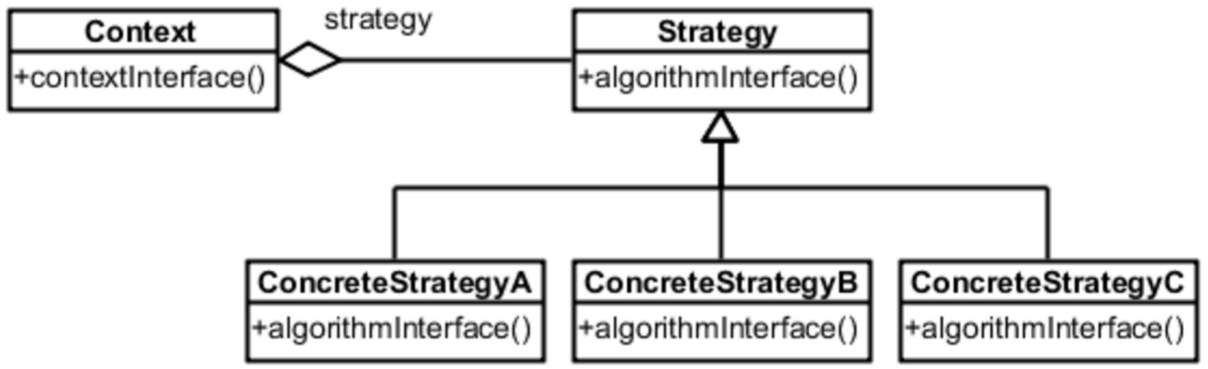
\includegraphics[width=0.7\textwidth]{strategy.png}
\end{center}

Context содержит стратегию как поле по интерфейсу Strategy. Когда пользователям что-то надо от Context, он делегирует запрос Strategy, и его исполняет объект конкретной стратегии, который сейчас у Context. Если стратегию надо поменять, то Context просто передают новый объект-стратегию, и он начинает перенаправлять запросы ему.

Хорошо это, если:

\begin{itemize}
    \item как в нашем примере с форматированием текста, имеется несколько разных алгоритмов, между которыми надо уметь легко переключаться;
    \item когда есть близкие по смыслу классы с разным поведением --- возможно, их можно зарефакторить так, чтобы само поведение вынести в стратегии, а сами классы склеить в один (Context в паттерне);
    \item когда класс всего один, но алгоритм сложный, состоит из нескольких этапов (которые можно вынести в private-методы), содержит вспомогательные данные (например, кеш), о которых не хочет знать контекст;
    \item в коде много условных операторов --- возможно, его можно зарефакторить, заменив условные операторы полиморфными вызовами стратегии.
\end{itemize}

\subsection{Детали реализации}

Первый и самый творческий момент при использовании паттерна <<Стратегия>> --- это проектирование его интерфейса (и интерфейса Context). Это надо сделать так, чтобы, с одной стороны, стратегии было остаточно информации для работы, с другой стороны, чтобы интерфейс не приходилось переделывать под каждую новую стратегию. В этом плане наиболее важно решить, как в стратегию передаётся необходимая для работы информация:

\begin{itemize}
    \item как параметры метода стратегии --- тогда стратегия может вообще ничего не знать про Context, но ей, скорее всего, придётся получать много лишних данных --- ведь не всем реализациям стратегии все аргументы потребуются;
    \item передавать сам Context в качестве аргумента, в надежде, что каждая стратегия сможет при необходимости спросить у него нужные ей данные --- это делает реализации стратегий более гибкими, но добавляет круговую зависимость между стратегией и контекстом, кроме того, заставляет контекст предоставлять интерфейс для доступа к данным, что плохо с точки зрения инкапсуляции.
\end{itemize}

Выбор, как обычно, зависит от конкретной ситуации и его должен сделать архитектор. Можно передавать аргументы и не в метод при вызове, а в конструктор стратегии, но обычно стратегия не имеет собственного состояния (кроме, быть может, кешей), так что это может быть плохой идеей. Почему --- стратегия может быть разделяемой: один объект-стратегия может обслуживать сразу много контекстов. Может быть разумно сделать стратегию приспособленцем из паттерна <<Приспособленец>> (о котором дальше) --- часть состояния, общую для всех обслуживаемых контекстов, стратегия хранит сама, часть передаётся извне при каждом вызове. И при этом есть единое место в системе, где каждый контекст может взять себе стратегию, когда ему надо.

Стратегия, кстати, может быть параметром шаблона, что особенно полезно в C++, поскольку там шаблоны раскрываются во время компиляции и это позволяет избежать оверхеда на виртуальные вызовы и хранение полей, неизбежного при использовании интерфейса Strategy. Так очень часто делает стандартная библиотека C++ --- например, аллокаторы часто передаются как параметры шаблона классам, которым они нужны. Естественно, такой приём можно использовать только тогда, когда стратегию не надо менять во время выполнения.

Ещё один немаловажный аспект применения этого паттерна --- при наивной реализации контекст будет падать, если стратегию случайно забыли выставить. С этим можно бороться, выставляя стратегию по умолчанию в конструкторе Context, либо просто if (стратегия установлена) вызвать-стратегию() else делать-что-то. Стратегия или поведение по умолчанию может обеспечивать базовую функциональность Context, а если пользователя это не устраивает, он может подсунуть ему свою стратегию.

И последнее замечание --- лямбда-функция тоже объект, и тоже созданный, чтобы инкапсулировать действие. Поэтому в современных языках лямбда-функции хорошо подходят для реализации простых стратегий, у которых всего один метод в интерфейсе. Благодаря замыканиям (closure), лямбда-функции даже могут иметь своё состояние и общаться с внешним миром.

\section{Задание на практику}

Надо расширить и уточнить модель компьютерной игры Roguelike из домашней работы, используя паттерны:

\begin{enumerate}
    \item <<Стратегия>> --- для поддержки различных поведений мобов. Поведений надо как минимум три:
    \begin{itemize}
        \item Агрессивное поведение, моб атакует игрока, как только его видит;
        \item Пассивное поведение, моб просто стоит на месте;
        \item Трусливое поведение, моб старается держаться на расстоянии от игрока.
    \end{itemize}
    \item <<Декоратор>> --- для поддержки временных эффектов, накладываемых на мобов и игрока. А именно, требуется спроектировать временный эффект конфузии, заставляющий персонажа двигаться в случайном направлении. Например, конфузия с некоторой небольшой вероятностью накладывается на моба при ударе (если он выжил), и дальнейшее движение моба <<корректируется>> случайным отклонением от выбранной им траектории. При этом архитектура должна позволять добавлять аналогичные эффекты.
\end{enumerate}

\end{document}
